%%%%%%%%%%%%%%%%%%%%%%%%%%%%%%%%%%%
%%  Datenbank
%%%%%%%%%%%%%%%%%%%%%%%%%%%%%%%%%%%

\section{Analyse back end}
%
%\subsection{Daten}
%In diesem Kapitel wird kurz erklärt welche Daten in der Datenbank, sowie in der später erklärten clientraw Dateien verarbeitet werden. Das Weather Display verarbeitet folgende Daten in für Menschen lesbare Produkte:
%\begin{itemize}
%\item Temperatur
%\item Gefühlte Temperatur (Windchill)
%\item Maximale, minimale gefühlte Temperatur (Windchill)
%\item Gefühlte Temperatur (Hitzeindex)
%\item Maximale, minimale gefühlte Temperatur (Hitzeindex)
%\item Maximale, minimale Temperatur 
%\item Windgeschwindigkeit
%\item Maximale Windgeschwindigkeit des Tages 
%\item Windrichtung
%\item Böengeschwindigkeit
%\item Maximale Böengeschwindigkeit des Tages
%\item Luftfeuchtigkeit
%\item Luftdruck
%\item Barometertrend letzte Stunde
%\item Regenmenge (täglich, monatlich, jährlich)
%\item Regenrate
%\item Taupunkt
%\item Wolkenhöhe
%\item Batteriestand
%\end{itemize}

% ################################
% Datenfluss, Text-Files
% ################################
\subsection{Datenzwischenspeicherung mittels Text-Files}
Die Daten werden von der Wetterstation an Weather-Display gesendet. Dieses verarbeitet die Daten und erstellt mehrere Text-Dateien (Tabelle~\ref{table:text-files}). Die Text-Dateien dienen WeatherDisplay Live als Grundlage für die Anzeigegrafiken. Neben den Text-Dateien sendet WeatherDisplay zudem einmal pro Minute sämtliche Werte an die MySQL-Datenbank.


\begin{table}[h!]
\centering
\begin{tabular}{|l|l|l|l|l|}
\hline
 Name			&  Anzahl Daten	& 	Zeitspanne  		& 	Intervall			\\ \hline
 Clientraw.txt 		&  174			&  	10min/20h zurück 	& 	5 Sekunden 		\\ \hline
 Clientrawextra.txt	&  767 			&  	24h zurück 		& 	1 Stunde 			\\ \hline
 Clientrawdaily.txt 	&  442 			&  	30 Tage zurück 	&  	1 Tag 			\\ \hline
 Clientrawhour.txt	&  673			&  	1h zurück 			& 	1 Minute 			\\ \hline
\end{tabular}
\caption{Von WeatherDisplay erstellte Text-Files}
\label{table:text-files}
\end{table}


\subsection*{Problem}
Der Inhalt der Text-Dateien kann nicht angepasst werden. Das bedeutet insbesondere, dass der Zeitabstand zwischen den Messungen nicht verringert werden kann. Zudem sind in diesen Text-Files nur die Daten des Multiwetter-Transmitters aufgeführt. Zusatzsensoren wie Pegel und Wassertemperatur sind nicht enthalten.

\subsection*{Lösungsansatz}
Während der Bachelor-Arbeit soll geprüft werden in wie weit die Daten aus den Text-Files für die Erstellung der neuen Anzeige-Elemente verwendet werden kann. 


% Abbildung (A3)
%\afterpage{ 
%\clearpage
%\KOMAoptions{paper=a3, paper=landscape} 
%\recalctypearea
%\newgeometry{left=30mm,right=30mm,top=30mm,bottom=50mm}
%
%\begin{figure}[h!p]
%	\centering
%	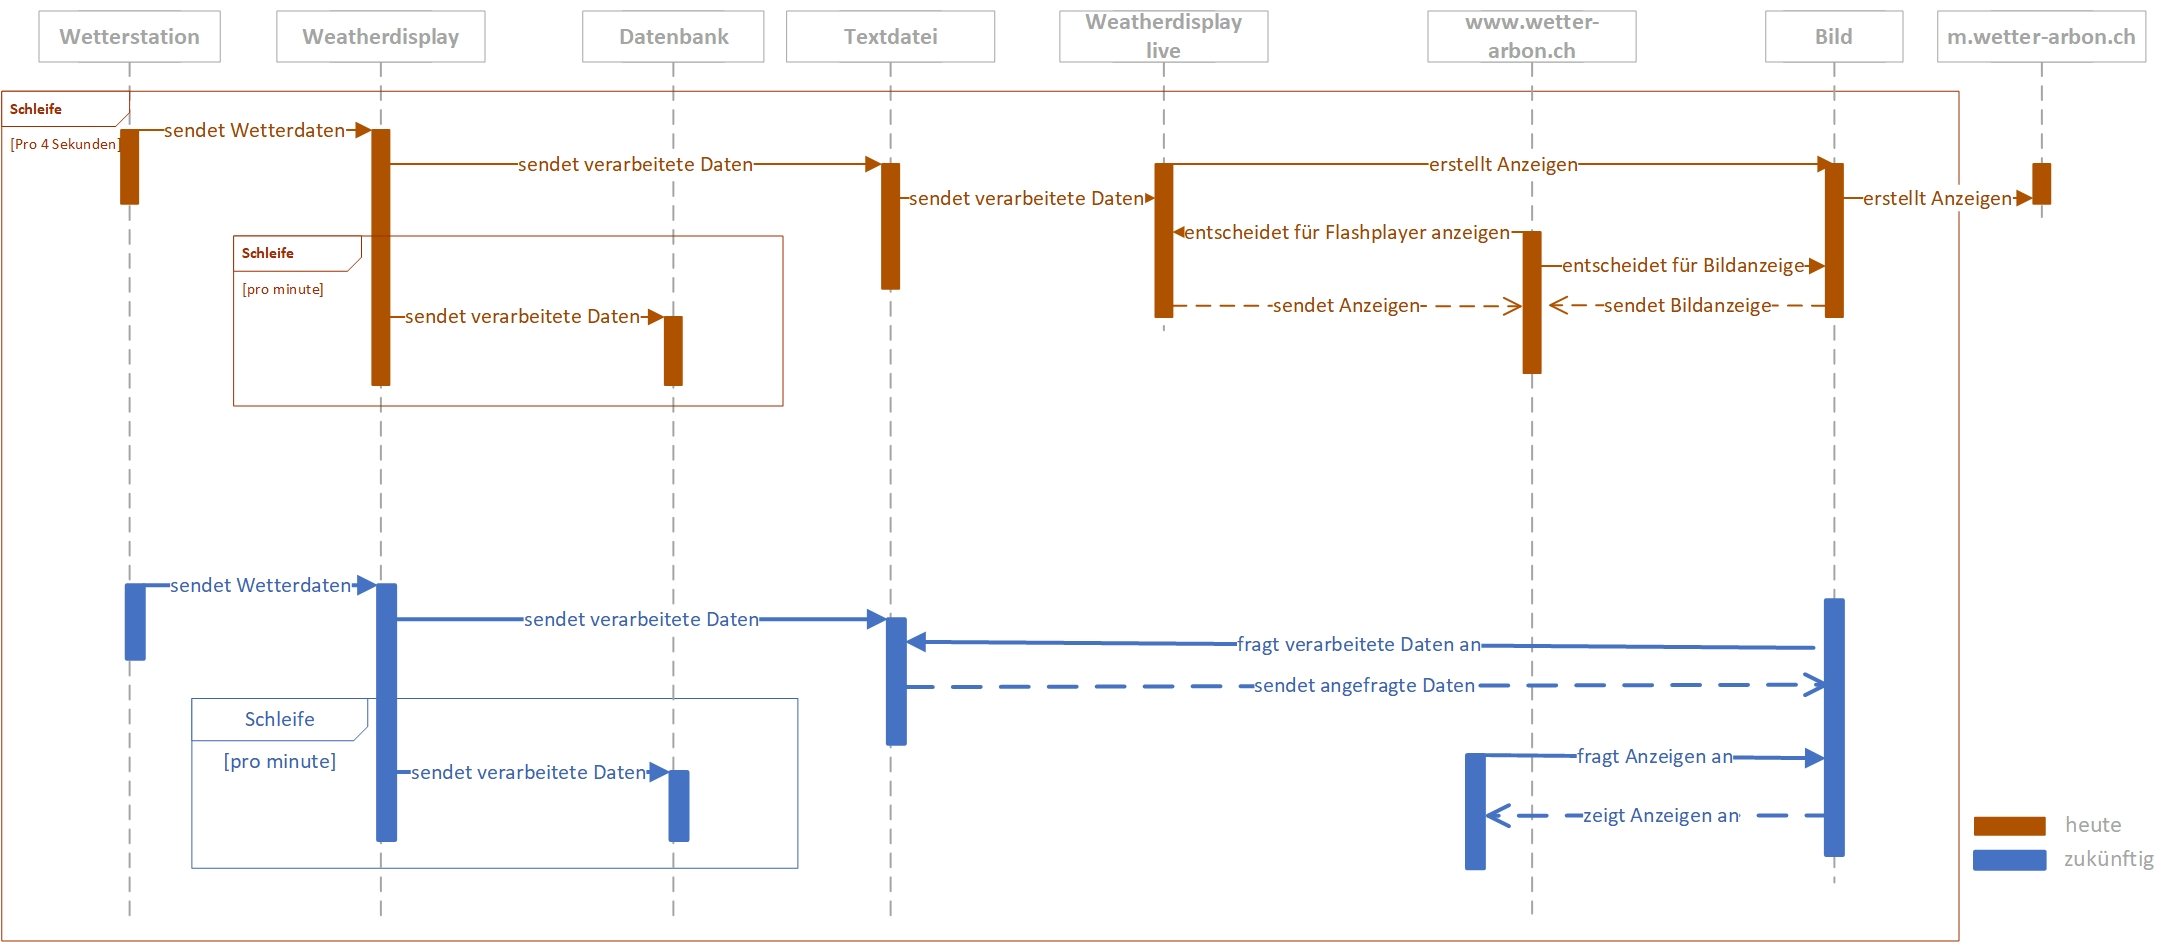
\includegraphics[width=2.5\linewidth]{img/Sequenzdiagramm_Wetter}
%	\caption{Ablauf von der Datenerfassung bis zur Anzeige}
%	\label{img:Sequenzdiagramm}
%\end{figure}
%
%
%\restoregeometry
%\KOMAoptions{paper=A4,pagesize}
%\recalctypearea
%}

% ################################
%Historische Daten (Datenbank)
% ################################
\subsection{Speicherung historischer Daten}
Um die Daten der Wetterstation zu speichern wird eine MySQL-Datenbank verwendet. Diese besteht aus mehreren Tabellen, die sich in Inhalt, Häufigkeit und Zeitraum unterscheiden, wie in Tabelle~\ref{table:db-tables} dargestellt. Auf der Webseite ist bereits eine Unterseite reserviert, um die historische Daten abfragen zu können. Bisher ist diese Funktion nicht implementiert.

\begin{table}[h!]
\resizebox{\textwidth}{!}{%
\begin{tabular}{|l|l|l|l|l|}
\hline
 Tabelle		&  Inhalt								& 	von  			& 	bis 			& 	Intervall\\ \hline
 tblgestern 	&  min und max Werte					&  	25.02.2005 	& 	14.07.2012 	& 	24h \\ \hline
 tblwellen		&  Pegel, Wellenhöhe, und Wassertemperatur 	&  	29.10.2013 	& 	28.01.2014  	& 	10min \\ \hline
 tblwind 		&  Windgeschwindigkeit- und Windrichtung 	&  	29.10.2013 	& 	28.01.2014 	&  	1min \\ \hline
 wx-data 		&  all von WXT gemessenen Werte			&  	25.02.2015 	&	heute  		& 	1min \\ \hline
 wx-pegel  	&  \multicolumn{4}{l|}{enthält keine Daten, da der Pegelsensor defekt ist} \\ \hline
\end{tabular}%
}
\caption{Vorhandene Daten in der Datenbank}
\label{table:db-tables}
\end{table}

\subsection*{Problem}
Um auf die Daten zugreifen zu können, müssen mehrere Tabellen abgefragt werden, was die Query und die Anzeige der Daten erschwert. Zudem fehlt ein Konzept welche Daten wo, wie und wie häufig gespeichert werden sollen.

\subsection*{Lösungsansatz}
Während der Bachelor-Arbeit soll ein Konzept erarbeitet werden, wie die Daten möglichst einfach in der Datenbank gespeichert und abgerufen werden können.


% ################################
% Datenmanagment und Datensicherung
% ################################
\subsection{Datenmanagement und Datensicherung}
Täglich fallen 93600 Datenpunkte an, diese Daten werden alle seit 2015 gespeichert und nicht ausgedünnt und für die Datenbank gibt es kein Backup beispielsweise auf eine externe Harddisk. Zusätzlich zur Datenbank werden auch die erwähnten clientraw Dateien benutzt um Anzeigen zu erstellen. Von diesen wird jährlich ein Backup erstellt und beim Hosting-service selber gespeichert.

\subsection*{Problem}
Ein weiterer Punkt sind die riesigen Mengen an Daten, diese verzögert eine Abfrage in der Datenbank enorm. zum anderen werden die seit dem erstellten Daten nicht auch in die "historische" Tabelle tblgestern abgelegt.


\subsection*{Lösungsansatz}
Hierfür wird vorgeschlagen die Datenbank igwetter openfile64Light so zu belassen, da diese für das CMS zuständig ist. Es wird eine neue Datenbank erstellt welche klarer strukturiert wird, hierbei sollten neue Tabellen entstehenen, wobei Daten ausgedünnt werden können um keinen unnötigen Speicherplatz zu belasten. Die Haupttabelle soll alle aktuelle Daten enthalten. Zusätzlich soll Tabelle erstellt werden mit zukünftigen und vorhandenen historischen Daten. Um die Übersichtlichkeit zu gewähren wird eine Tabelle mit Maximal sowie Minimal Daten erstellt. Die Zeitabstände, in der die Daten gelöscht bzw. zu historischen Daten werden, müssen noch mit den Mitgliedern der IG-Wetter abgesprochen werden. Ein weiterer Punkt auf der Liste sollten die zukünftigen Backups sein, d.h. diese sollten nicht als .txt sonder auch als .sql File gespeichert sein damit im Falle eines Datenverlustes die Datenbank einfach wiederherzustellen ist.



